\section{Обзор предметной области}
\label{sec:survey}
\subsection{Постановка задачи моделирования видеотрафика
с переменной битовой скоростью}

Пусть есть некоторая видеопоследовательность ---
последовательность изображений в цифровом RAW-формате.
Данная последовательность подвергается сжатию с помощью
некоторого видеокодера, сконфигурированного с целью
сохранения качества видео при переменном размере кадра.

В данной работе в качестве стандарта видеокодера
используется H.264~\cite{h264spec}, один из распространённых
стандартов сжатия видео. Кадровая частота, размер кадров (разрешение)
и цветовое разрешение тестовой последовательности известны.

С точки зрения моделирования видеотрафика, сжатый видеопоток
можно представить как последовательность из $N$ кадров
размера $S_i,~i=1\dots N$. Внутренняя структура сжатого
кадра не рассматривается. Кадры, тем не менее, разделены
на три типа в зависимости от использования и типе межкадрового
предсказания (англ. inter-frame prediction)~\cite{salomoncomp}.
В стандарте H.264~\cite{h264spec} предусмотрено разбиение каждого
кадра на прямоугольные области одинакового размера (макроблоки),
для каждой из которых индивидуально определяется тип и наличие
предсказания, но с ограничением, определяемым типом всего кадра:

\begin{itemize}
    \item I-кадры (также называются ``ключевыми'', англ. intra-frames).
        Содержат только макроблоки, сжатые независимо от макроблоков
        других кадров.
    \item P-кадры (``разностные'' кадры, англ. predicted frames).
        Могут содержать как макроблоки, сжатые независимо от других
        кадров, так и макроблоки, сжатие которых осуществлялось с
        опорой на другой предшествующий I- или P-кадр.
    \item B-кадры (``двунаправленные'' кадры, англ. bi-predicted frames).
        Могут содержать макроблоки следующих типов: предсказанные с опорой
        на другой I-, P-, B-кадры или с опорой на два кадра любого в
        общем случае типа, один из которых предшествует текущему,
        а другой следует за текущим кадром.
\end{itemize}

Как правило, в видеокодеках используется некоторая техника
разностной импульсно-кодовой модуляции (англ. differential
pulse-code modulation, DPCM)~\cite{sklarbook}, предполагающая некоторую
процедуру предсказания текущего макроблока по множеству других.
Выбор макроблоков, на основе которых производить предсказание,
и является критерием типизации макроблоков и кадров.

Наличие ``опорных'' кадров позволяет существенно ускорить
время получения произвольного кадра в потоке и ``быстрой
перемотки с показом'', поскольку в этом случае декодирование
можно начинать с ближайшего ``опорного'' I-кадра.
Однако предсказание лишь на основе текущего кадра не
позволяет использовать временн\'{у}ю избыточность
видеопотока~\cite{salomoncomp}.

``Разностные'' кадры позволяют
экстраполировать временн\'{о}е поведение видеопотока
и получить более точное предсказание. ``Двусторонние''
кадры заменяют временн\'{у}ю экстраполяцию интерполяцией,
что приводит к повышению точности предсказания.
Использование межкадрового предсказания требует
усложнения процедуры декодирования ввиду необходимости в
буферизации как декодированных (I- и P-кадры), так и
сжатых кадров (для использования двустороннего предсказания).

Цепочки кадров разных типов между соседними I-кадрами называются
GOP (англ. Group of Pictures). Типовая цепочка, используемая
в кодеком x264 (реализацией стандарта H.264)~\cite{x264page},
имеет вид

$$
\mathtt{IBBPBBPBBPBBPBBPBBPBBPBBP}.
$$

В ней B-кадры
ссылаются на два ближайших I- или P-кадра и независимы
между собой. Данная структура схематически изображена
на Рис.~\ref{fig:ipb_frames}.

\begin{figure}[h]
    \begin{center}
        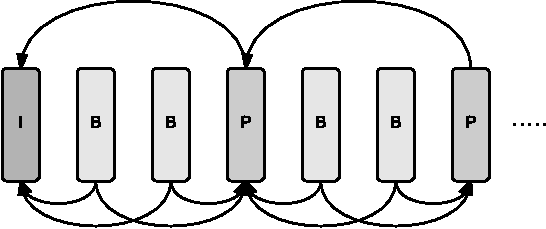
\includegraphics[width=0.7\textwidth]{ipb_chart.pdf}
    \end{center}
    \caption{Схематическое изображение структуры сжатого потока
    для кодека x264 по умолчанию}
    \label{fig:ipb_frames}
\end{figure}

Значительная часть моделей видеотрафика~\cite{survey2013} разделяют
сжатый поток кадров разного типа на подпотоки и моделируют
их независимо, получая результирующий поток путём последующего
совмещения подпотоков в соответствии с требуемой схемой.
При таком подходе основной задачей моделирования является
моделирование подпотока одного типа.

В данной работе рассматривается задача моделирования потока
P-кадров, в котором каждый последующий кадр ссылается на
предыдущий. Схема данного потока проиллюстрирована на Рис.~\ref{fig:ippp_frames}.

\begin{figure}[h]
    \begin{center}
        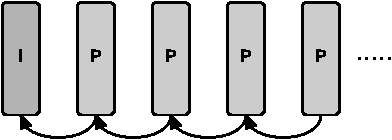
\includegraphics[width=0.55\textwidth]{ippp_chart.pdf}
    \end{center}
    \caption{Схематическое изображение моделируемой структуры сжатого потока
    для кодека x264}
    \label{fig:ippp_frames}
\end{figure}

Таким образом, в задачи данного дипломного проекта входит:

\begin{itemize}
    \item анализ особенностей сжатого VBR-трафика видеоконференций;
    \item обзор существующих моделей VBR-видеотрафика и анализ
        целесообразности их использования при моделировании
        трафика видеоконференций;
    \item реализация набора существующих моделей VBR-видеотрафика
        и методики их адаптации к особенностям трафика видеоконференций;
    \item обзор методов сравнительного анализа моделей;
    \item сравнительный анализ результатов моделирования VBR-трафика
        видеоконференций.
\end{itemize}

\subsubsection{Формальное определение задачи}
\label{sse:task}
\hspace{3pt}

Приведённые ограничения позволяют предложить формальное определение задачи
моделирования выхода видеокодера с переменной битовой скоростью.
Пусть $S = \{S_i\} _{i=1}^N$ --- последовательность размеров P-кадров на выходе видеокодера.
$S$ можно рассматривать как реализацию случайного процесса $\Sigma$~\cite{randomprocesses}
\begin{itemize}
    \item с дискретными состояниями (размеры кадров)
    \item дискретного по времени ($\tau$ -- интервал следования кадров -- единица измерения времени)
    \item неизвестной структуры
\end{itemize}

Задача моделирования видеокодера может быть сформулирована в терминах
теории о вероятностных процессах как определение случайного
процесса $\Sigma$ по набору его реализаций $S$.

Эта задача не имеет решения, поэтому исследователи видеотрафика
прибегают~\cite{characteristics2013} к эвристическим методам определения структуры
случайного процесса. Задача моделирования видеотрафика может быть
сформулирована следующим образом: предложить случайный процесс
$\Sigma'(S)$, реализации $S'$ которого будут ``соответствовать''
реализации $S$ по набору характеристик. Таким образом,
каждая тестовая видеопоследовательность рассматривается
как реализация случайного процесса, которая используется
для ``адаптации'' модели $\Sigma'$ под особенности
конкретного видео.

\subsection{Анализ особенностей трафика видеоконференций}
%\hspace{3pt}

С точки зрения специалистов в области сжатия видео~\cite{survey2013},
видеоданные могут быть условно разделены на классы по
следующим параметрам:

\begin{itemize}
    \item ``активность'' (количество движения) в кадре. Численно 
        эту характеристику можно оценить путём получения разности
        двух последовательных кадров;
    \item ``локальность'' движения. Сосредоточенность энергии
        разностного кадра в конкретных областях кадра;
    \item наличие ``смены сцен''. Смена сцены --- это эвристически
        определяемая резкая перемена освещения, смена плана,
        и тому подобное. Обычно определяется~\cite{scenedetection} как превышение
        энергии разностного кадра некоторого порога;
    \item геометрические размеры кадра (разрешение)
    \item зашумлённость
    \item требования к качеству сжатого видео: глубина цвета,
        разрешение, соотношение сигнал-шум (PSNR)~\cite{salomoncomp}.
\end{itemize}

Обычно видео разделяют на подтипы по происхождению,
каждый из которых обладает собственным набором признаков.
Для видеопоследовательностей разных классов требуются
различные конфигурации видеокодека или даже разработка
собственного кодека, приспособленного под данный класс видео.

\begin{table}[ht]
    \caption{Сравнение отличительных особенностей несжатого видеотрафика разного происхождения}
    \centering
    \begin{tabular}{| c | c | c | c | c | c |}
\hline
                      & Спорт    & CCTV     & Conference  & Кино       & Casual  \\
\hline
\specialcell{Активность\\в кадре}    &  Высокая &  Малая   &  Малая      & Переменная & Высокая \\
\hline
\specialcell{Локальность\\движения}  &  Низкая  &  Высокая &  Высокая    & Переменная & Низкая  \\
\hline
Зашумлённость         &  Низкая  &  Высокая &  Переменная & Низкая     & Высокая \\
\hline
Смена сцен            &  Частая  &  Редкая  &  Отсутствие & Частая     & Частая  \\
\hline
    \end{tabular}
    \label{tab:videotypes}
\end{table}

В данной дипломной работе объектом моделирования является
сжатый трафик видеоконференций, который в несжатом виде
характеризуется следующими признаками (Таблица~\ref{tab:videotypes}):

\begin{itemize}
    \item малая активность в кадре;
    \item локальный характер движения;
    \item отсутствие смены сцен;
    \item умеренная зашумлённость.
\end{itemize}

\subsection{Использованное при моделировании тестовое множество}
%\hspace{3pt}

Вышеприведённые особенности несжатого трафика видеоконференций
были критерием отбора тестовых видео. Тестовое множество было
составлено из десяти видеозаписей, половина из которых
находилась в базе тестовых видео Государственного Университета
Аризоны~\cite{traceas}, которая используется специалистами в области
сжатия видео в качестве ``общего знаменателя'', который позволяет
сравнивать различные алгоритмы сжатия видео на одинаковых
видеопоследовательностях. Следующие видеозаписи были
признаны подходящими для использования в качестве
записей видеоконференций:

\begin{itemize}
    \item Akiyo
    \item Foreman
    \item Miss-America
    \item Suzie
    \item Claire
\end{itemize}

Данные видеозаписи имеют низкое разрешение (примерно 300x300 пикселей)
и маленькую продолжительность (примерно 300-500 кадров при кадровой
скорости 25 кадров в секунду). С помощью встроенной веб-камеры были
самостоятельно получены более продолжительные тестовые видеопоследовательности
различного разрешения и качества:

\begin{itemize}
    \item Boris
    \item RomanL
    \item RomanM
    \item RomanS
    \item RomanSQ
\end{itemize}

\begin{table}[ht]
\caption{Характеристики тестового множества}
\centering
\begin{tabular}{| c | c | c | c | c |}
\hline
              & Разрешение & Длительность & FPS & QP \\ \hline
Akiyo         & 176x144    & 12s          & 25  & 5  \\ \hline
Foreman       & 176x144    & 12s          & 25  & 5  \\ \hline
Miss-America  & 176x144    & 6s           & 25  & 5  \\ \hline
Suzie         & 176x144    & 6s           & 25  & 5  \\ \hline
Claire        & 176x144    & 20s          & 25  & 5  \\ \hline
Boris         & 480x320    & 2h           & 30  & 11 \\ \hline
RomanL        & 1280x720   & 10m          & 30  & 5  \\ \hline
RomanM        & 640x480    & 20m          & 30  & 5  \\ \hline
RomanS        & 320x240    & 10m          & 30  & 5  \\ \hline
RomanSQ       & 320x240    & 10m          & 30  & 25 \\ \hline
\end{tabular}
\label{tab:videos}
\end{table}

Характеристики сжатого видео представлены в таблице~\ref{tab:videos}.
В данной таблице используются следующие обозначения:
\begin{itemize}
    \item QP (англ. Quantization Parameter) --- это параметр кодера x264,
        значение которого прямо пропорционально степени сжатия исходного видео
        и, соответственно, обратно пропорционально качеству декодированного;
    \item FPS (англ. Frames Per Second) --- кадровая скорость видео. Период
        следования кадров есть величина, обратная FPS.
\end{itemize}


\subsection{Критерии сравнительного анализа моделей}
%\hspace{3pt}

Формулировка задачи (раздел~\ref{sse:task}) предусматривает
сравнение тестовой видеопоследовательности с синтезированной.
Сравнение последовательностей (трейсов, англ. trace) осуществляется
по тем параметрам, которые играют значение при непосредственной
передаче трафика по сети. Можно выделить две группы сравнительных
характеристик: статистические характеристики и характеристики качества
обслуживания.

Из статистических характеристик интерес представляет распределение
размеров кадров и автокорреляционная структура случайного процесса.

При определении моментов распределения размеров кадров усреденение
по статистическому ансамблю реализаций заменяется на усреднение
по времени. Таким образом, неявно предполагается эргодическая
структура случайного процесса~\cite{ergodic}.

Сравнение характеристик качества обслуживания основывается
на предположении, что точная модель должна демонстрировать
такие же показатели синтетического трейса при передаче по
сети, что и исходная последовательность.

В данной работе следующие характеристики видеопоследовательностей
используются для сравнения тестовых видеопоследовательностей
со сгенерированными:

\begin{itemize}
    \item Статистические характеристики
        \begin{itemize}
            \item гистограмма размеров кадров
            \item первые два момента распределения размеров кадров
            \item автокорреляционная функция последовательности размеров кадров
        \end{itemize}

    \item Характеристики качества обслуживания
        \begin{itemize}
            \item потери при переполнении буфера
            \item задержка
            \item джиттер
        \end{itemize}
\end{itemize}

В разделе~\ref{sec:modelcomp} подробно описана
методика сравнительного анализа моделей на основе
вышеприведённых критериев.

\subsection{Особенности сжатого видеотрафика}
\label{sse:traces}
%\hspace{3pt}

Первым шагом к моделированию сжатого видеотрафика конкретного
типа является исследование его статистических особенностей.
В ходе данного исследования было установлено, что типовая
гистограмма распределения размеров кадров имеет
куполообразный характер. Типовая гистограмма приведена на
рисунке~\ref{fig:romanbell}.

\begin{figure}[h]
    \begin{center}
        \includegraphics[width=\textwidth]{roman_bell.pdf}
    \end{center}
    \caption{Типовая гистограмма распределения размеров кадров (для видео RomanS)}
    \label{fig:romanbell}
\end{figure}

Подобный характер зависимости позволяет аппроксимировать
распределение размеров кадров хорошо изученными аналитическими
распределениями, способными малым числом параметров описывать
большое количество тестовых видеопоследовательностей.
В исследовательских публикациях в таком качестве используется
Гамма-распределение~\cite{heymansourcemodels},
распределение Пирсона типа V~\cite{lazarismodelling},
логарифмическое нормальное распределение~\cite{Krunz95atraffic} и
отрицательное биномиальное распределение~\cite{heymanATM}.

Второй обнаруженной особенностью исследуемого типа видеотрафика
является зависимость автокорреляционной структуры видеопоследовательности
от разрешения и степени квантования видео. В соответствии с рисунком~\ref{fig:acfs},
скорость убывания функции автокорреляции обратно пропорциональна качеству
видеопоследовательности. Природа данного феномена остаётся невыясненной;
коэффициент автокорреляции последовательности инвариантен к её произведению на скаляр,
поэтому меньший размер сжатого кадра как таковой не может являться
причиной изменения функции автокорреляции.

\begin{figure}[h]
    \begin{center}
        \includegraphics[width=\textwidth]{acfs_resolution.pdf}
    \end{center}
    \caption{Автокорреляционная функция для видео разного качества}
    \label{fig:acfs}
\end{figure}

В целом в научных публикациях~\cite{raey} утверждается, функция автокорреляции
для трафика видеоконференций хорошо аппроксисмируется экспонентой. Настоящая
работа готова подтвердить этот результат для видео плохого качества,
но не для высококачественного трафика видеоконференций. На текущий момент
качество (разрешение, степень квантования) передаваемого трафика исследуемого типа
остаётся низким. Однако необходимость в моделировании трафика видеоконференций
высокого качества может привести к разработке моделей с неэкспоненциальной
автокорреляционной структурой.

\newpage
\subsection{Описание существующих подходов к моделированию VBR-видеотрафика}
\label{sse:survey}

В данном подразделе приведено краткое описание основных подходов
к моделированию видеотрафика, описаны их особенности и степень
применимости к моделированию конкретного подкласса видеотрафика ---
трафика видеоконференций.

``Хорошая'' модель видеотрафика должна отражать его статистические
характеристики и демонстрировать такие же характеристики качества
обслуживания при передаче по сети произвольной конфигурации.
Одним из наиболее важных статистических характеристик
видеотрафика является функция автокорреляции (англ. autocorrelation function, ACF)
размеров кадров.
Точное отражение автокорреляционных характеристик видеотрафика ---
сложная задача, потому что в общем случае видеопоследовательности
имеют как краткосрочные (англ. Short-Range Dependent, SRD), так
и долгосрочные (англ. Long-Range Dependent, LRD) зависимости.
С точки зрения автокорреляционной структуры, случайные процессы
могут быть разделены на три типа: независимые, SRD- и LRD-процессы.
У независимых процессов автокорреляция равна нулю при любом
ненулевом смещении. Функция автокорреляции SRD-процессов
убывает экспоненциально. ACF LRD-процессов убывает медленнее~\cite{raey}.

Существующие подходы к моделированию видеотрафика можно условно
разделить на пять классов~\cite{survey2013}:

\begin{itemize}
    \item Авторегрессионные модели: очередной размер кадра
        определяется некоторой функцией от предыдущих кадров
        некоторого временн\'{о}го окна;
    \item Модели, основанные на марковских процессах: марковские
        процессы используются для представления изменений
        в битовой скорости, размеров кадров, сцен или GOP-ов
        (англ. Group of Pictures);
    \item Самоподобные и дробные ARIMA модели: способны отражать
        долгосрочные зависимости в моделируемом трафике;
    \item Вейвлетные модели: вейвлетные преобразования используются
        для того, чтобы отражать как краткосрочные, так и долгосрочные
        зависимости в моделируемом трафике;
    \item Прочие модели: немногочисленные не принадлежащие к
        приведённым классам модели, такие, как модель M/G/$\infty$
        и TES-модель.
\end{itemize}
\hspace{5pt}

Далее приведена краткая характеристика каждого из подходов.

\subsubsection{Авторегрессионные модели}
\hspace{3pt}

Особенностью авторегрессионных случайных процессов является
явная зависимость очередного элемента реализации от фиксированного
количества предыдущих значений. Простой авторегрессионный процесс может
быть описан следующим образом~\cite{ars2004, survey2013}:

\begin{equation}
    S_i = \sum_{k=1}^p a_k S_{i - k} + e_i,
\end{equation}

где $p$ -- порядок авторегрессионного процесса, $a_1, a_2, \dots a_p$ -- коэффициенты
авторегрессии. Последовательность $e_i$ состоит из независимых, равномерно
распределённых случайных величин, которая иногда называется остаточным процессом.
Таким образом, каждый последующий элемент в простом авторегрессионном процессе
есть взвешенная сумма $p$ предыдущих элементов и случайного остатка, в качестве
которого часто используют аддитивный белый гауссовский шум (АБГШ) с нулевым средним
и оценённым на основе тестовой последовательности дисперсией. Параметры авторегрессии
соответствуют оценённым коэффициентам автокорреляции тестовой последовательности.

Такая авторегрессионная модель способна точно отражать автокорреляционную структуру
входной последовательности, но её использование затруднено в случае, когда
распределение размеров кадров распределено по неаддитивному закону, потому что
в таком случае распределение размеров кадров на выходе модели отличается
от распределения остаточного процесса.

Искажённое распределение размеров кадров отсутствует в другом типе
авторегрессионных моделей: дискретной авторегрессионной модели~\cite{heymanATM}.
Основное её отличие от обычной авторегрессионной модели состоит
в том, что вместо линейной комбинации предыдущих значений
в качестве очередного значения выбирается либо новое сгенерированное
значение ``остаточного процесса'', либо конкретное значение из предыстории.
Данная модель реализована в дипломной работе и подробно описана в
подразделе~\ref{sse:darp}.

Некоторые модификации авторегрессионных моделей предусматривают
дополнительные усовершенствования для использования остаточного
процесса требуемого типа, например, модель Gamma AR~\cite{gar},
использующая Гамма-распределение остаточного процесса, или
Gamma-Beta AR~\cite{gbar} с Гамма-Бета распределением размеров
кадров остаточного процесса. Другие усовершенствования призваны
учитывать смену сцен, как, к примеру, Frame-Based AR~\cite{Krunz95atraffic}
или Nested AR~\cite{nestedar}.

В целом, все авторегрессионные модели способны отражать краткосрочные
зависимости, так как функция автокорреляции для этого семейства
случайных процессов убывает экспоненциально, однако неспособны
отражать долгосрочные зависимости. Авторегрессионные модели
часто использовались для моделирования именно трафика видеоконференций~\cite{ars2004}
и, в целом, хорошо справляются с этой задачей.

Из преимуществ этого подхода следует отметить его относительную простоту
и способность моделировать широкий класс видеопоследовательностей
для видеоконференций при помощи небольшого числа параметров.
Эти модели не подходят, однако, для самоподобного трафика с
долгосрочными зависимостями или для трафика со сложной структурой
(смена сцен, различные типы кадров и пр.). Эти сложности
обнаружили необходимость в создании более сложных моделей,
преимущественно для моделирования кинематографического видео
(см. таблицу~\ref{tab:videotypes}).

\subsubsection{Марковские модели}
\hspace{3pt}

Марковские модели предполагают использование марковского
случайного процесса (цепи Маркова)~\cite{markovchains}.
Цепи Маркова часто используются в качестве процесса
``верхнего уровня'', контролирующего параметра некоторого
другого случайного процесса.
Текущее состояние марковского случайного процесса зависит
лишь от его предыдущего состояния.

Текущее состояние ``доминирующего процесса'' зависит
только от предыдущего состояния. Марковский процесс
часто контролирует параметры некоторого другого процесса,
например, авторегрессионного~\cite{mmar}.

Марковские модели можно разделить по значению состояния цепи
маркова в данной модели:

\begin{itemize}
    \item состояние определяет размер группы кадров (GOP);
    \item состояние определяет тип кадра (I- B- или P-);
    \item цепь Маркова контролирует переходы между режимами
        активности в сценах;
    \item состояние непосредственно определяет размер кадра.
\end{itemize}
\hspace{3pt}


Далее приведены примеры использования состояний в марковских
цепях для различных целей:
\begin{itemize}
    \item размер кадра: Markov Renewal Process (MRP)~\cite{heymanATM};
    \item смена сцен: Markov-Modulated AR~\cite{mmar};
    \item смена сцен: Markov-Modulated Gamma Model~\cite{mmg};
    \item смена сцен, типы кадров: Scene-Based Markov Model~\cite{scenemm}.
\end{itemize}

Б\'{о}льшая часть марковских моделей была создана для учёта
смены сцен в видеопоследовательностях, поэтому они оказываются
избыточными в рамках данной дипломной работы в силу специфики
сжатого трафика видеоконференций (см. таблицу~\ref{tab:videotypes}).

Как и авторегрессионные, марковские модели обладают экспоненциальным
характером убывания функции автокорреляции, что зачастую
делает их непригодными для моделирования трафика с долгосрочными
зависимостями.

Преимуществами марковских моделей является возможность
``тонкой настройки'' модели под каждое конкретное видео.
С другой стороны, подбор параметров модели (например,
подбор границ активности сцен) является сложной задачей;
некоторые авторы занимались подбором границ активности
сцен вручную~\cite{mmar}.

Марковская модель на основе MRP~\cite{heymanATM} была
выбрана как подходящая для исследуемой задачи, так как
она моделирует кадры одного типа без учёта смены сцен.
В подразделе~\ref{sse:marksimple} приведено подробное
описание этой модели, а в подразделе~\ref{sse:markkmeans}
описано предложенная в данной работе модификация модели.

\subsubsection{Самоподобные и другие LRD-модели}
\hspace{3pt}

Самоподобные модели были созданы для того, чтобы
моделировать трафик с сильными зависимостями.
LRD (Long-Range Dependent) процесс является самоподобным,
если для любых значений смещения и после усреднения по
блокам любой длины коэффициент автокорреляции остаётся
неизменным.

Long-Range Dependence (зависимость с большой памятью - авт.) ---
явление, при котором текущие значения случайного процесса
сильно коррелированы со значениями, удалёнными во времени.

Степень зависимости во времени характеризуется параметром
Хёрста $0.5 < H < 1$. Чем больше этот коэффициент, тем в большей
степени в последовательности выражены долгосрочные зависимости.
Этот параметр оценивается по тестовой
последовательности и подаётся на вход самоподобному случайному процессу.

Самоподобные модели разрабатывались для кинематографического видеотрафика.
Характерной чертой таких процессов является степенная зависимость
функции автокорреляции от смещения~\cite{selfsimilar}. Такие процессы
не в состоянии точно отражать краткосрочные зависимости
в моделируемом трафике, а для трафика видеоконференций типичное
значение параметра Хёрста -- $0.6-0.75$~\cite{raey}, что делает
неоправданным их применение в данной работе.

Было проведено самостоятельное определение параметра Хёрста для
видео из тестового множества. Оказалось, что видео плохого качества
действительно имеет малые значения параметра Хёрста, а видео хорошего
качества -- большие. Это подтверждается визуальным сопоставлением функций
автокорреляции для видео различного качества, приведённым на рисунке~\ref{fig:acfs}.

\subsubsection{Вейвлетные модели}
\hspace{3pt}

Модели, основанные на вейвлетном преобразовании~\cite{salomoncomp},
позволяют точно отражать как краткосрочные, так и долгосрочные зависимости
в моделируемом трафике. Их использование требует компетенции в области
обработки сигналов.

Общий шаблон использования вейвлетных преобразований в моделировании
видеотрафика заключается в следующем~\cite{survey2013, wavelet}:

\begin{itemize}
    \item К исходной последовательности применяется вейвлетное преобразование;
    \item Производится оценка корреляции коэффициентов этого преобразования;
    \item Генерируются новые коэффициенты преобразования на основе построенной корреляционной модели;
    \item Применяется обратное вейвлетное преобразование, в результате которого получается синтезированный трейс.
\end{itemize}
\hspace{2pt}

Особенности и преимущества вейвлетных подходов состоят в следующем:
\begin{itemize}
    \item Не требуется дополнительной надстройки для учёта смены сцен;
    \item Точно отражает как близкие, так и дальние зависимости моделируемого трафика;
    \item Дальние зависимости по времени переходят в близкие
        зависимости коэффициентов преобразования, что существенно
        упрощает работу с долгосрочно зависимым трафиком.
\end{itemize}
\hspace{2pt}

Учитывая тот факт, что в данной работе предполагается отсутствие
смены сцен и долгосрочных зависимостей в моделируемом трафике,
использование вейвлетных методов было признано избыточным.
Как показал дальнейший анализ, моделирование сжатого трафика
для видеоконференций высокого качества может потребовать использование
подобных методов.

\subsubsection{Прочие модели}
\hspace{3pt}

Среди не вписывающихся в предложенную классификацию моделей
можно выделить модель на основе метода TES (англ. Transform-Expand-Sample)~\cite{tesmodel},
и модель на основе M/G/$\infty$-процесса~\cite{mginfty}.

Модель на основе TES способна моделировать любой тип видеотрафика,
однако требует использования проприетарной утилиты TESTool и поэтому
исключена из рассмотрения в данной работе.

M/G/$\infty$-модель создавалась для весьма специфической цели:
было замечено, что функция автокорреляции некотрых последовательностей
лучше всего аппроксисмируется не показательной и не степенной,
а некоторой промежуточной функцией:

\begin{itemize}
    \item ACF для LRD-моделей: $\rho(k) = k^{-\beta} = e^{-\beta \log k}$;
    \item ACF для марковских моделей: $\rho(k) = e^{-\beta k}$;
    \item наиболее подходящая ACF: $\rho(k) = e^{-\beta \sqrt{k}}$.
\end{itemize}

Автокорреляция такого типа наблюдается в теории массового обслуживания
для процессов типа M/G/$\infty$~\cite{bertsekas}, что было решено использовать для
получения последовательности размеров кадров с необходимой автокорреляционной
структурой.

Для процесса M/G/$\infty$ авторы аналитически вывели функцию плотности
вероятности для распределения времени обслуживания
G так, чтобы количество занятых серверов обладало требуемыми
автокорреляционными характеристиками. Осуществляется
моделирование такой системы, на выходе получается количество
занятых серверов в каждый момент времени.
Далее производится
преобразование полученной случайной величины таким образом,
чтобы свести распределение вероятностей к целевому (Gamma/Pareto)~\cite{mginfty}.

Функция автокорреляции для трафика видеоконференций хорошо моделируется
экспоненциальным законом, поэтому данная модель также не была использована.
